\section{Experiments and Evaluation}
\subsection{Environment}
We used the game "Breakout" from the Gym toolkit \cite{brockman2016openai} as an
environment for the agent. Breakout is a game in which the player controls a
paddle to bounce the ball towards some blocks. Every block the ball touches gets
destroyed, if no block is left the player wins. If the ball reaches the bottom
end of the screen without being redirected by the paddle again, the player
loses.

The reinforcement learning agent learning and playing the game was Proximal
Policy Optimization (PPO) \cite{raffin2019stable}. PPO is an on-policy
algorithm, that uses an actor critic approach. We used the implementation of the
stablebaselines3 package \cite{raffin2019stable} as a starting point, and
modified it to our needs.

\subsection{Dimension reduction}
Our first set of experiments featured the basic dimension reduction method,
without the modifications for compression. We were looking to verify that the
required reconstruction information was present within the lower dimensional
representation created by the feature extractor. The qualitative results can be
seen in Figure \ref{fig:baseline_MSE} (it should be noted that the images came
from the training set). \\

\begin{figure}[H]
    \centering
    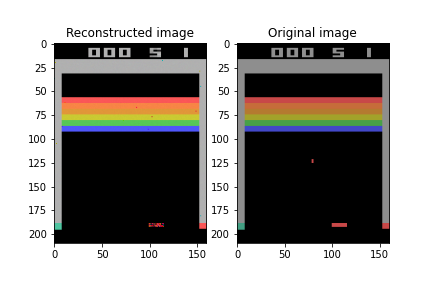
\includegraphics[width=0.6\textwidth]{images/orig_reconstructed0.0.png}
    \caption{Baseline method (no compression) with decoder trained on MSE for 10,000 iterations}
    \label{fig:baseline_MSE}
\end{figure}


\subsection{Compression}
Now we added the compression loss to the training of the RL agent, equation
\ref{eq:RL_Training_Loss} and trained the agent with this loss function. We
modified the $\alpha$ value, looking at the performane of the decoder. An alpha
of $1e-4$ seemed to work best, therefore we chose this value for an
extended run over $1e5$ add epochs. Tested on an independently created test
dataset, this resulted in an entropy of 1.7 bits per latent dimension, if the
latent values get rounded to 3 digits. The actual bitrate given by the
cross-entropy \ref{eq:BitRate} is higher however, since we need to choose a
fixed distribution for encoding and transmission of the latents. As for training
we chose a normal distribution with mean 0 and learned variance, we also use
this for testing. The expected variance per dimension was estimated by the mean
per dimnesion over the whole test dataset. However the cross entropy over the
test dataset was infinity. A visual investigation of the latent values showed
that while the entropy of the latent values was low, some of the values deviated
of 0 significantly, (in the order of 100), which led to a probability of nearly
0 and a logprob of -infinity.

After training the RL Agent, the decoder was trained for $2e5$ epochs. This
resulted in an MSE Loss of 1895. As discussed in \ref{sec:Introduction}, MSE
Loss is not a good metric for performance, since it gives each pixel the same
value. Therefore we investigated some images. An example can be seen in figure
\ref{fig:final_agent}.
\begin{figure}[H]
    \centering
    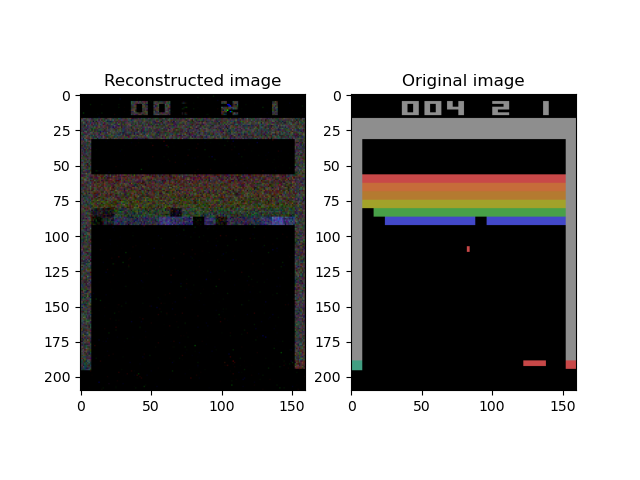
\includegraphics[width=0.6\textwidth]{images/orig_reconstructed_final_agent.png}
    \caption{Final agent}
    \label{fig:final_agent}
\end{figure}

\subsection{Latent Loss Scheme}
As discussed in section \ref{sec:Introduction}, L2 Loss might be suboptimal and
we introduced a latent loss scheme \ref{sub:Distortion} as an alternative.
Training a decoder with the latent loss scheme showed an decrease in image
quality compared to L2 Loss scheme, see figure \ref{fig:baseline_MSE_latent}
(also from the training set).

\begin{figure}[H]
    \centering
    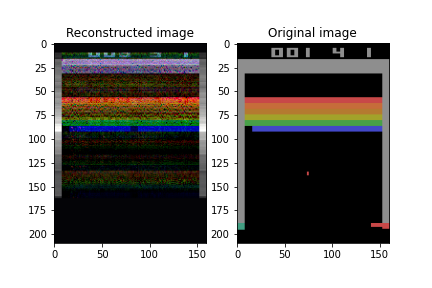
\includegraphics[width=0.6\textwidth]{images/orig_reconstructed_rl3.0.png}
    \caption{Baseline method (no compression) with decoder trained on MSE for 10,000 iterations, then latent MSE for 10,000 iterations}
    \label{fig:baseline_MSE_latent}
\end{figure}

\subsection{Adaptive Alpha}
When we implemented our custom loss function with static $\alpha$, several
rudimentary tests were done to verify that the model behaved as expected. One
such test involved varying $\alpha$: we expected that a lower value would
prioritize task performance, while a higher value would prefer a lower bitrate.
However, we found this was not the case: there seemed to be just as much
variation between independent tests of the same $\alpha$ as changing $\alpha$.
Given our hypothesis for where the problem lay (see \ref{sub:Adaptive_Alpha}),
we developed the adaptive $\alpha$ scheme. However, initial results showed no
improvement and we were forced to move this to Future Work.

\subsection{Pretrained agents}
Another idea was that adding the compression loss to the RL agent from the
beginning on was a too large constrain for the agent to learn anything.
Therefore, we tried to fix this by first pretraining the agent, and then adding
the compression loss to the agent. On the one hand, the additional compression
loss reduced the entropy but on the other hand, the decoder didn't learn
anymore after the training, so this procedure showed no improvements.


